\PassOptionsToPackage{usenames,dvipsnames}{xcolor}
\documentclass[twocolumn,twocolappendix]{aastex63}

% Add your own macros here:
\pdfoutput=1 %for arXiv submission
%\usepackage{amsmath,amssymb,amstext}
\usepackage{amsmath,amstext}
\usepackage[T1]{fontenc}
\usepackage{apjfonts}
\usepackage{ae,aecompl}
\usepackage[utf8]{inputenc}
\usepackage[figure,figure*]{hypcap}
\usepackage{natbib}
\usepackage{url}
\usepackage{listings}

\urlstyle{same}

\usepackage{lineno}
\linenumbers
%\modulolinenumbers[2]

\newcommand{\placeholder}[1]{\textit{PLACEHOLDER: #1}}


% header settings
\shorttitle{Tomographic binning optimization}
\shortauthors{Author A et al.\ (LSST~DESC)}

% ======================================================================

\begin{document}
\title{The LSST DESC 3x2pt Tomography Optimization Challenge}
\collaboration{1000}{The LSST Dark Energy Science Collaboration (LSST DESC)}
\noaffiliation

% paper leads

\author[0000-0001-9789-9646]{Joe Zuntz}
\affiliation{Institute for Astronomy, University of Edinburgh, Edinburgh EH9 3HJ, United Kingdom}

\author[0000-0001-7956-0542]{Fran\c{c}ois Lanusse}
\affiliation{AIM, CEA, CNRS, Universit\'e Paris-Saclay, Universit\'e Paris Diderot, Sorbonne Paris Cit\'e, F-91191 Gif-sur-Yvette, France}

%main partticipants and text contributors  (alphabetical)
\author{Bela Abolfathi}
\noaffiliation

\author[0000-0002-4598-9719]{David Alonso}
\affiliation{Astrophysics, University of Oxford, DWB, Keble Road, Oxford OX1 3RH, UK}


\author{Abby Bault}
\noaffiliation

\author[0000-0003-4383-2969]{Cl\'{e}cio R. Bom}
\affiliation{Centro Brasileiro de Pesquisas F\'isicas, Rua Dr. Xavier Sigaud 150, 22290-180 Rio de Janeiro, RJ, Brazil}
\affiliation{Centro Federal de Educa\c{c}\~{a}o Tecnol\'{o}gica Celso Suckow da Fonseca, Rodovia M\'{a}rcio Covas, lote J2, quadra J - Itagua\'{i} (Brazil)}


\author{Massimo Brescia}
\affiliation{INAF - Osservatorio Astronomico di Capodimonte, via Moiariello 16, I-80131, Napoli Italy}

\author{Adam Broussard}
\noaffiliation

\author[0000-0002-1590-6927]{Jean-Eric Campagne}
\affiliation{Universit\'e Paris-Saclay, CNRS/IN2P3, IJCLab, 91405 Orsay, France}

\author[0000-0002-3787-4196]{Stefano Cavuoti}
\affiliation{INAF - Osservatorio Astronomico di Capodimonte, via Moiariello 16, I-80131, Napoli Italy}
\affiliation{INFN - Sezione di Napoli, via Cinthia 21, I-80126 Napoli, Italy}
\affiliation{Department of Physics ``E. Pancini'', University of Naples Federico II, via Cintia, 21, I-80126 Napoli, Italy}


\author{Eduardo S. Cypriano} $^3$
\affiliation{Universidade de S\~ao Paulo, IAG, Rua do Mat\~ao 1225, S\~ao Paulo, SP, Brazil}


\author{Bernardo M. O. Fraga}
\affiliation{Centro Brasileiro de Pesquisas F\'isicas, Rua Dr. Xavier Sigaud 150, 22290-180 Rio de Janeiro, RJ, Brazil}

\author{Eric Gawiser}
\noaffiliation


\author[0000-0002-0226-9893]{Elizabeth J. Gonzalez} $^{4,5}$.
\affiliation{Instituto de Astronom\'{\i}a Te\'orica y Experimental (IATE-CONICET), Laprida 854, X5000BGR, C\'ordoba, Argentina.}

\affiliation{Observatorio Astron\'omico de C\'ordoba, Universidad Nacional de C\'ordoba, Laprida 854, X5000BGR, C\'ordoba, Argentina.}


\author{Dylan Green}
\noaffiliation

\author{Peter Hatfield}
\noaffiliation

\author{David Kirkby}
\noaffiliation


\author{Alex Malz}
\noaffiliation

\author{Andrina Nicola}
\noaffiliation

\author{Erfan Nourbakhsh}
\noaffiliation

\author{Andy Park}
\noaffiliation

\author{Anze Slosar}
\noaffiliation

\author{Gabriel Teixeira}
\affiliation{Centro Brasileiro de Pesquisas F\'isicas, Rua Dr. Xavier Sigaud 150, 22290-180 Rio de Janeiro, RJ, Brazil}

\author{Angus Wright}
\noaffiliation

% minor contributions and/or text writers (alphabetical)


\begin{abstract}
In this paper we present the results of the DESC 3x2pt tomography challenge,
which aims to compare strategies for optimizing the photometric binning required
for the main LSST 3x2pt analysis. This task is made particularly delicate in the
context of a metacalibrated lensing survey, as only the photometry from the
bands  included in the metacalibration process (riz and potentially g) can be
used to define this tomographic binning. Using a set of realistic simulations
including true galaxy redshifts and simulated photometry, the goal of the
challenge is to propose a bin assignment strategy that maximizes the overall
Figure of Merit of a 3x2pt analysis. This setting is idealized as it ignores
spectroscopic completeness  issues for the training sample, but complex enough
to address the main question of binning optimization. Based on the challenge
dataset, we review and compare the different methods that have been proposed by
participants. We find that even from this limited photometry information,
various methods are able to yield binning schemes that achieve high figure-of-merit scores.
\end{abstract}

\keywords{methods: statistical -- dark energy  -- large-scale structure of the universe}

%\accepted{}
%\submitjournal{the Astrophysical Journal Supplement}


%\tableofcontents%-----------------------------
%===========================
% BEGINNING OF THE MAIN TEXT
%===========================

\section{Introduction}
Weak gravitational lensing (WL) has emerged over the last decade as a powerful
cosmological probe \citep{cfhtlens,des,kids,hsc}.  WL
uses measurements of coherent shear distortion to the observed shapes of galaxies
to track the evolution of large-scale gravitational fields.  It measures the integrated
gravitational potential along lines of sight to source galaxies, and can thence constrain
the laws of gravity, the expansion history of the Universe, and the history and growth
of cosmic structure.

WL has proven especially powerful in combination with galaxy clustering measurements,
which can measure the density of matter up to an unknown bias function.  The high signal
to noise of such measurements and the relative certainty of the redshift of these foreground
samples breaks degeneracies in the systematic errors that affect WL.

The \emph{3x2pt} method has become the standard method for performing this combination.
In this method, two-point correlations are computed among and between two samples, the shapes of 
background (source) galaxies and the locations of foreground galaxies, which trace foreground
dark matter haloes.  The three combinations (source-source, source-lens, and lens-lens) are
measured in either Fourier or configuration space, and can be predicted from a combination of 
perturbation theory and simulation results.  The method has been used in the Dark Energy Survey, DES
\citep{des-3x2pt}, and to combine Baryon Oscillation Spectroscopic Survey, BOSS, with the Kilo-Degree 
Survey, KiDS \citep{kids-3x2pt}.

Most lensing and 3x2pt analyses have been performed \emph{tomographically}, 
binning galaxies by redshift.
This approach captures almost all the available information in lensing data, since it measures
an integrated effect and so galaxies nearby in redshift probe very similar fields.  For photometric
foreground samples it is similarly near-lossless, since redshift estimates of such galaxies have
large uncertainties\footnote{Spectroscopic foreground samples may be more likely to see significant 
gains from moving beyond spectroscopic methods.}.  Binning galaxies by approximate redshift lets us 
model galaxy bias, intrinsic alignments, and other systematic errors en masse in a more tractable way.
While fully 3D methods have been proposed and prototyped \citep{kitching,more}, the tomographic 
approach remains the standard within the field.

Tomographic 3x2pt measurements will be a key science goal in the upcoming \emph{Stage IV} surveys,
including the Rubin Observatory \citep{rubin} and the Euclid and Roman space telescopes \citep{euclid,roman}.

In this paper we discuss and evaluate methods for assigning objects to tomographic bins, and 
specifically the impact
of using a limited set of color bands to make those assignments, motivated by requirements of using the
metacalibration method for galaxy shape measurement to limit biases.  Tomographic methods have been 
explored before in \citet{jain} and \citet{kitching2019}.  In this paper we describe the results of a 
challenge using simulated Rubin-like data with a range of methods submitted by different teams.  We explore how many tomographic bins we can effectively generate using only a subset of bins, and compare methods submitted to the challenge.

In \autoref{sec:motivation} we explain the need for methods that work on limited sets of bands in the context of upcoming lensing surveys.  \textbf{Complete structure...}

\section{Motivation}
\label{sec:motivation}

The methodology used to assign galaxies to bins faces special challenges when we use a particularly
effective approach for measuring galaxy shear, called \emph{metacalibration} (metacal),
which was introduced in \citet{sheldonhuff} and developed further in \citet{sheldon}.
In metacal, galaxy images are deconvolved from the point-spread function (PSF), sheared, and
reconvolved before measurement, allowing one to directly compute the response of a metric
to underlying shear and correct for it when computing two-point measurements.  This can
almost completely remove errors due to model and estimator (noise) bias from WL data, at least
when PSFs are well-measured and oversampled by the pixel grid.

Furthermore, metacal provides a solution to the pernicious and general problem of
\emph{selection biases} in WL.  Measurements of galaxy shear are known to have noise-induced errors
that are
highly covariant with those on other galaxy properties, including size and, most importantly, flux/
magnitude.  It follows that a cut (or re-weighting) on galaxy magnitudes, or on any quantity derived
from  them, will induce a shear bias since galaxies will preferentially fall either side of the cut
depending on their shear.  Within metacal, we can solve this problem by performing the cut on both
sheared variants of the catalog, and measuring the difference between the post-cut shear in the two
variants.  In DES the corrected biases were found up to around 3\%, far larger than
the requirements for the current generation of surveys \citep{des-y1-cat}.

In summary: metacal allows us to correct for significant selection biases, but only if all selections
are performed using only bands in which the PSF is measured well enough for deconvolution to be
performed.  For Rubin, this means using only the $r$, $i$, $z$, and perhaps $g$ bands.  In this work we
therefore study how well we can perform tomography using only this limited photometric information.  In
particular, this limitation prevent us from using the most obvious method for tomography,
and computnig a complete photometric probability density function (PDF) for each galaxy and assigning
a bin using the mean or peak of that PDF.

Simulation methods can also be used to correct for selection biases, provided that they match the
real data to high accuracy.  If we determine that limiting the bands we can use for tomography results
in a significant decrease in our overall signal-to-noise, outweighing the gain from the improved shape
calibration then this might suggest moving to rely more on such methods\footnote{One can account for
residual shear estimation uncertainty during parameter estimation by marginalizing over an unknown
factor.  Widening the prior on this factor decreases the overall constraining power of the analysis.}.


\section{Challenge Design}

The Dark Energy Science Collaboration (DESC) Tomographic Challenge was launched in May 2019 and 
advertised among the LSST cosmology community, though it was open to outside entrants.

In the challenge, participants assigned simulated galaxies to tomographic bins,
using only their (g)riz bands and associated errors.  Their goal was to maximize the cosmological
information in the final split data set; this is generally acheived by separating different bins by 
redshift as much as possible.  Particpants were free to optimize or simply select nominal (target) 
redshift bin edges from their training sample, but in either case had to classify galaxies into the 
different bins.

\subsection{Philosophy}

Since this was a preliminary challenge designed to explore whether it is possible \emph{in theory}
to use only (g)riz for tomography, we chose to simplify several aspects of the data.  In realistic 
situations we will have access to limited sized training sets for WL photometric redshifts, since 
spectra are time-consuming to obtain.  These training sets will also be highly incomplete compared
to full catalogs, especially at faint magnitudes where spectroscopic coverage is sparse.  In this
challenge we avoided both these issues -- the training samples we provided (see below) were comparable
in size to the testing sample, and drawn from the same population.  Given this, the challenge
represents a best-case scenario -- if no method succeeded on this easier case then more realistic
cases would probably be impossible.

Despite these simplifications, the other aspects of the challenge and process were designed to be
as directly relevant as possible to the particular WL science case we focus on.  The data set
was chosen to mimic the population, noise, and cuts we will use in real data (see \autoref{sec:data}, 
and the metrics were designed to be as close to the science goals as possible, rather than a lower
level representation (see \autoref{sec:metrics}). The data set was also large enough to pose a 
reasonably realistic test of methods at the large data volume required for upcoming surveys, where
$10^9$ -- $10^{10}$ galaxies will be measured.

The challenge was open to any entrants, not just those already involved in DESC, but it was
advertised primarily through Rubin, and so is perhaps best described as semi-public.
Participants tested and ran their methods locally, but submitted code to be run as part of a central
combined analysis on the NERSC supercomputing facility.  No prize was offered apart from recognition.


\subsection{Data}
\label{sec:data}

We run challenge entries on two data sets, CosmoDC2 and Buzzard, each of which is split into training, 
validation, and testing components.  In each case participants were supplied with the training and 
validation data, and the testing data was kept secret for final evaluation. In each case the three
data sets were random sub-selections of the full data sets, with the training and testing sets 25\% of 
the full data each and the validation 50\%. In practice many entrants trained on a subset of
this, so to make the final evaluation phase tractable we trained on 1M objects for both data sets.

We used the second Buzzard catalog for two reasons.  First, to check the significance of
an issue with galaxy colour assignments in CosmoDC2, described below.  And second, to check
for over-fitting in the design of models themselves, and thus to determine whether two
reasonable but different galaxy populations can be optimized by the same methods; this will
tell us whether our conclusions might be reasonable for real data. We discuss correlations
between metrics in Section \ref{sec:metric-results}.

Each of these data set come from cosmological simulations which provide truth values of galaxy magnitudes
and sizes.  We simulate and add noise to the objects as described below.

\subsubsection{CosmoDC2}

The CosmoDC2 simulation was designed to support the Dark Energy Science
Collaboration and is described in detail in \citet{cosmodc2}.  It covered 440
deg${}^2$ of sky, and used the dark matter particles from the Outer Rim
simulations \citep{outer_rim}.  The UniverseMachine \citep{universe_machine}
simulations were then used, with the GalSampler technique \citep{galsampler},
in a combination of empirical and semi-analytic
methods, to assign galaxies with a limited set of specified properties to halos.

These objects were then matched to outputs of the Galacticus model
\citep{galacticus}, which generated complete galaxy properties and which was run
on an additional DESC simulation, AlphaQ, and included all the LSST bands.  The
simulation is complete to $r=28$, and contains objects up to redshift 3.  We
include the ultra-faint galaxies in the simulation, not assigned to a specific
halo.

After the post-processing and selections described below, and a cut to a specific geographic region, 
we used around 36M objects from the CosmoDC2 simulations.

One limitation of the CosmoDC2 catalogs we used, found during the challenge,
was that the matching to Galacticus led to only a limited number of SEDs being
used at high redshifts, and thus too many galaxies in the simulations sharing
similar characteristics at these redshifts, such as colour-colour relations.
It was unknown whether this limitation would have any practical impact on the challenge,
and was one of the reasons for adpoting the additional Buzzard catalog.

\subsubsection{Buzzard}

The Buzzard catalog was developed to support Dark Energy Survey Year 1 (DES-Y1)
data analysis, and is described in detail in \citet{buzzard}.  It used dark
matter simulations from L-GADGET2 \cite{lgadget} and then added galaxies using
the {\sc AddGals} algorithm \citet{addgals}, which matches a set of galaxy
property probability densities to data using sub-halo abundance matching. 
Buzzard galaxies extend to around redshift 2.3, and were shown to be a good
match (after appropriate selections) to DES-Y1 observable catalogs.  Magnitudes
using the LSST band passes were provided in the catalog.

After the post-processing and selections described below, and a cut to a
specific geographic region,  we used around 20M objects from the Buzzard
simulations.


\subsubsection{Post-processing}

We add noise to the truth values in the extra-galactic catalogs to simulate real observations.
In each case we simulate observations corresponding to the first year Rubin observations
using the DESC {\sc TXPipe} framework, following the methodology of \citet{ivezic_jones_lupton}
and assuming the numerical values for telescope and sky characteristics therein.

In both simulations we add two cuts to approximately simulate the selection used in a real
lensing catalog.  In both cases we apply a cut on the combined $riz$ signal to noise of
$S/N > 10$, and a size cut $T / T_\mathrm{psf} > 0.5$, where
$T$ is the trace $I_{xx} + I_{yy}$ of the moments matrix and measures the squared radius of the
galaxy compared to that of the PSF.



\subsection{Metrics}
\label{sec:metrics}

In this challenge we use only a lensing source (background) population, since the metacal requirements
do not apply to the foreground lens sample. We do, however, calculate 3x2pt metrics using the
same source and lens populations, both because this scenario is one that will be used in some analyses,
and because clustering-like statistics of lensing samples are important for studies of intrinsic
alignments. We use two different sets of metrics, one based on the over signal to noise of the spectra 
derived from the samples, and one based on a figure-of-merit for the constraints that would be obtained 
using them.  \textbf{Discuss how correlated these turn out to be here}.  

For each bin $i$ generated by a challenge entry, we make a histogram of the true redshifts 
of each galaxy assigned to the bin.  This is then used as our number density $n_i(z)$ in the metrics 
below. Both metrics reward bins that can
cleanly separate galaxies by redshift, since this reduces the covariance between the samples. No
method can perfectly separate them, so good methods reduce the tails of $n_i(z)$ that overlap with 
neighbouring bins.

We developed two implementations of each of these metrics, one using the Core Cosmology Library 
\citep{ccl} and one the JAX Cosmology Library \citep{jax-cosmo}, which provides differentiable theory 
predictions using the JAX library \citep{jax}.  In production we use the latter since it provided a
more stable calculation of metric 2.

Metric 1 would be approximately measurable on real data without performing a full cosmology analysis,
whereas metric 2 would be the final output of such an analysis.  We therefore simulate performance
tests at multiple stages in the wider process.


\subsubsection{Metric 1: Sigal-to-noise}
Our first metric is the total signal-to-noise ratio of the power spectrum derived from the assigned
$n_i(z)$ values:
\begin{equation}
    S = \mu^{T} C^{-1} \mu
\label{eq:snr}
\end{equation}
where $\mu$ is a stack of the theoretical predictions for the $C_\ell$ spectra for each tomographic 
bin, in turn, and $C$ a Gaussian estimaate of the covariance between them, as described in
\citet{wl-review} and summarized in \autoref{app:theory}.   We compute this metric for lensing alone, clustering alone, and the full 3x2pt combination.

\subsubsection{Metric 2: Figure-of-merit}

Metric 2 uses a figure of merit (FOM) based on that presented by the Dark Energy Task Force (DETF) \citep{detf}.  We 
use the inverse area of a Fisher Matrix ellipse, which approximates the size in two axes 
of the posterior PDF one would obtain on analysing the spectra:
\begin{align}
    F &= \left( \frac{\partial \mu}{\partial \theta} \right)^T C^{-1} \left( \frac{\partial \mu}{\partial \theta} \right), \\
    S &= \frac{1}{2 \pi \sqrt{\det{([F^{-1}]_{p_1, p_2})}}}
\label{eq:fom}
\end{align}
where $[F^{-1}]_{p_1, p_2}$ extracts the 2x2 matrix for two parameters.  We use both the original
DETF variant in which $p_1 = w_0, p_2 = w_a$, representing the constraining power on dark energy 
evolution, and a version in which $p_1 = \Omega_c$ and $p_2 = \sigma_8$, representing constraining
power on overall cosmic structure amplitude and its evolution.




\subsection{Infrastructure}
\begin{itemize}
    \item Pull request submissions
    \item Data at NERSC
\end{itemize}


\subsection{Control Methods}

Two control methods were used to test the challenge machinery and metrics.
The first method randomly assigned galaxies to each tomographic bin, resulting
in bins which each had the same $n(z)$, on average.  Using this method, we expect
that increasing the number of bins should not increase any metric, since bins are
maximally correlated.  We find this to be true for all our metrics.

Second, we use a method which uses only the $i$-band to select tomographic bins,
splitting galaxies in equal-sized bins in this magnitude. We expect only a small
increase in metrics with the number of bins, and also that the addition of the $g$-band
should make no difference to metrics.  Again, we find this to be true.

One additional method was submitted to the challenge with the caveat that it could
never be applied to real data and should therefore considered a form of control method.
This method was {\sc Utopia}, which found, for each object in the testing data, the
nearest neighbour object in the training sample.  The high density, completeness, and
representativeness of our training set made this possible; realistics spectroscopic training
sets are too sparse.  The method performed well, as expected, 
but was not the highest scoring overall.


\section{Methods}

\subsection{ {\sc RandomForest} } \label{sec:randomforest}
This method was submitted by the challenge organizers and used a random
forest algorithm to assign galaxies.

Random forests \citep{breiman2001} train a collection of individual \emph{decision trees},
each of which consists of a set of bifurcating comparisons in which different features in
the data (in this case, magnitudes and errors) are compared to criterion values to choose
which branch to follow.  Each ``leaf'' (end comparison) selects a classification bin for
an input galaxy, and the tree is trained to choose comparison features and comparison values
which maximally split the discrimination at each step, and in final leaf purity.

Since decision trees tend to over-fit data, random forests generate a suite of decision
trees, each randomly choosing a subset of features on which to train at each bifurcation.
An average over the trained trees is taken as the overall classification.

In this implementation we chose nominal bin edges by splittng ensuring equal numbers of training set 
objects were in each bin, and then trained the forest to map magnitudes, magnitude errors, and
galaxy sizes to bin indices.  We use the {\sc scikit-learn} implementation of the random forest
\citep{scikit-learn}.


% Please describe your methods with some very general / high level background theory
% and a focus on the spsecific implementation.  Add any citations you like with bibtex in
% paper.bib
% Feel free to rename your method, but please leave a comment explaining so that I can do the
% same in the tables.

\subsection{ {\sc LSTM} } 
\label{ClecioLSTM} 
Methods \ref{ClecioLSTM} - \ref{ClecioEnsemble} were
submitted by a team of authors CRB, BMOF, GT, ESC, and EJG.  All were built using TensorFlow, and
chose bin edges such that an equal number of galaxies is assigned to each bin, and trained the
network using the galaxies' magnitudes and colours. 

The LSTM method uses a Bidirectional Long Short Term Memory network to assign galaxies to redshift
bins.
 
Recurrent Neural Networks (RNNs)\citep{schuster, medsker, pascanu} are a type of NN capable of
analyzing sequential data, where data points have a strong correlation with their neighbours. Long
Short Term Memory (LSTM) units are a particular type of RNN capable of retaining relevant
information from previous points while at the same time removing unnecessary data. This is achieved
through a series of gates with learnable weights connected to different activation functions to
balance the amount of data retained or removed.
 
In some cases, relevant information can come both from data points coming before or after each point
being analyzed. In such cases, two LSTMs can be combined, each going in a different direction, to
create effectively a bidirectional LSTM cell \citep{schuster}.
 
In this implementation, we chose bin edges such that an equal number of galaxies is assigned to each
bin, and trained the network using the galaxies' magnitudes and colours. The net was implemented
using Tensorflow and Keras. The Deep model is composed of a series of convolutional blocks (1d
convolutional layer with a tanh activation followed by a MaxPooling layer) followed by a
bidirectional LSTM layer and a series of fully connected layers. 

\subsection{ {\sc Autokeras LSTM}}
Autokeras \citep{autokeras} is an AutoML system based on Keras. Given a general neural network
architecture and a dataset, it searches for the best possible detailed configuration for the problem
at hand. 
 
We started from the basic architecture and bin assignment scheme mentioned in Section
\ref{ClecioLSTM} and let Autokeras search for the configuration that results in the lowest
validation loss. We kept the order of the layer blocks fixed, i.e., convolutional blocks,
bidirectional LSTM, and Dense blocks. We let the other hyperparameters free, such as the number of
neurons,  Dropout rates, maxpooling layers, the number of convolutional filters, and strides.


\subsection{ {\sc LGBM} }
This method uses a Light Gradient Boosted Machine (LightGBM) \citep{lgbm} to assign galaxies to
redshift bins.
 
LightGBM uses a histogram-based algorithm that assigns continuous feature values to discrete bins
instead of other pre-sort-based algorithms for decision tree learning. LightGBM also grows the trees
leaf-wise, which tends to achieve lower losses than level-wise tree growth. This method tends to
overfit for small data so that a \textit{max\_depth} parameter can be specified to limit tree depth.

 
In this implementation, we chose bin edges such that an equal number of galaxies is assigned to each
bin, and trained the network using the galaxies' magnitudes and colours.

 
\subsection{ {\sc TCN}}
This method uses a Temporal-Convolutional (TCN) \citep{baitcn} network to assign galaxies to redshift
bins.
 
Recurrent Neural Networks (such as LSTMs) are considered to be the state-of-the-art model for
sequence modelling. However, research indicates that certain convolutional architectures can achieve
human-level performance in these tasks \citep{dauphin}.
 
TCNs are Fully Convolutional Networks with causal convolutions, in which the output at time
\textit{t} is convolved only with elements of time \textit{t} and lower in the previous layer. This
new approach prevents leakage of information from the future to the past. This simple model has one
disadvantage, in that it needs a very deep architecture or large filters to achieve a long history
size. 
 
By using dilated convolutions, where a fixed step is introduced between adjacent filter taps, the
receptive field of the TCN can be increased without increasing the number of convolutional filters.
Furthermore, residual blocks \citep{he} are also used to stabilize deeper and larger networks. These
modifications cause TCNs to have a longer memory than traditional RNNs with the same capacity,  and
also require low memory for training.
 
We used the Keras implementation of TCN \citep{kerastcn} and chose bin edges such that an equal
number of galaxies is assigned to each bin, and trained the network using the galaxies' magnitudes
and colours. 

\subsection{ {\sc CNN} } 
This method uses an optimized Convolutional Neural Network (CNN) to assign
galaxies to redshift bins. 
 
CNNs \citep{lecun2015deep} are layers inspired in pattern recognition types developed in mammals' brains.
They consist of kernels that are convolved with the data as it flows through the net. CNN-based
models have emerged as state-of-the-art in several computer vision tasks, such as image
classification and pose estimations, as well as having applicability in a range of different fields.
 
We combine the Convolutional layers are with dimensionality reduction (pooling layers) and different
activation functions. Here, we used Autokeras to optimize a general convolutional architecture,
using the galaxies' magnitudes and colours to assign them to redshift bins, which were chosen such
that an equal number of galaxies were assigned to each.


\subsection{ {\sc Ensemble} } 
\label{ClecioEnsemble} 
This method combines different neural network
architectures to assign galaxies to redshift bins.
 
Deep Ensemble models combine different neural network architectures to obtain better performance
than any of the nets alone. In this method, we used the Bidirectional LSTM optimized by Autokeras, a
ResNet \citep{resnet} and a Fully Convolutional Network (FCN) \citep{fcn}. The predictions of these
models were averaged to get the final predicted bin. 
 


\subsection{ {\sc ComplexSOM} }
The {\tt ComplexSOM} method implements an additional optimization layer on the
methodology used by {\tt SimpleSOM}.

Let ${\sf C}^{\rm group}_\ell$ be the matrix containing all auto- and
cross-power spectra between members of a large set of galaxy samples (called
``groups'' here). We can compress this large set into a smaller set of samples
(called ``bins'' here), by combining different groups. Let ${\sf A}$ be the
assignment matrix determining these bins, such that $A_{\alpha,i}=1$ if group
$i$ is assigned to bin $\alpha$, and 0 otherwise. In that case, the redshift
distribution of bin $\alpha$ is given by $N_\alpha(z)=\sum_i
A_{\alpha,i}n_i(z)$, where $n_i(z)$ is the redshift distribution of group $i$.

Defining the normalized assignment matrix ${\sf B}$ as
\begin{equation}
B_{\alpha,i}=A_{\alpha,i}\frac{\int dz\,n_i(z)}{\sum_j A_{\alpha,j}\int dz\,n_j(z)},
\end{equation}

${\sf C}^{\rm group}_\ell$ is related to the matrix of cross-power spectra
between pairs of bins via:
\begin{equation}
{\sf C}^{\rm bin}_\ell={\sf B}\,{\sf C}^{\rm group}_\ell\,{\sf B}^T.
\end{equation}

The rationale behind the {\tt ComplexSOM} method is based on the observation
that, while ${\sf C}^{\rm group}_\ell$ is a slow quantity to calculate for a
large number of groups, ${\sf B}$ and therefore ${\sf C}^{\rm bin}_\ell$ are
very fast. Thus, given an initial set of groups characterizing the
distribution of the full sample in colour space, ${\sf C}^{\rm group}_\ell$
can be precomputed once, and used to find the optimal assignment matrix ${\sf
B}$ that maximizes the figure of merit in Equation \ref{eq:fom},
which can be written in terms of ${\sf C}^{\rm bin}_\ell$ alone as

\begin{equation}\label{eq:fom_tr}
F_{\theta\theta'}=\sum_\ell f_{\rm sky}\frac{2\ell+1}{2}{\rm Tr}\left[\partial_\theta{\sf C}^{\rm bin}_\ell({\sf C}^{\rm bin}_\ell)^{-1}\partial_{\theta'}{\sf C}^{\rm bin}_\ell({\sf C}_\ell^{\rm bin})^{-1}\right].
\end{equation}

Note that the general problem of finding the matrix ${\sf B}$ that optimally
compresses the information on a given parameter has an analytical solution in
terms of Karnhunen-L\^oeve eigenvectors \citep{astro-ph/9603021}. However, the
assignment matrix used in this case has the additional constraints that it
must be positive, discrete and binary (i.e. groups are either in a bin or they
are not). Thus, finding the absolute maximum figure of merit would involve a
brute-force evaluation of all matrix elements $A_{\alpha,j}$, which is an
intractable $N_{\rm bin}^{N_{\rm group}}$ problem. We thus parametrize ${\sf
A}$ in terms of a small set of continuous parameters, for which standard
minimization routines can be used. In particular we use $N_{\rm bin}-1$
parameters, given by the edges of the redshift bins, and a group is assigned
to a bin if its mean redshift falls within its edges. We also explored the
possibility of ``trashing'' groups if less than a fraction $p_{\rm in}$ of its
redshift distribution fell within its preassigned bin, treating $p_{\rm in}$
as an additional free parameter. We found that adding this extra freedom did
not translate into a significant improvement in the final level of data
compression.

Once the SOM has been generated, the {\tt ComplexSOM} method proceeds as
follows. First, the full SOM is distilled into a smaller set of ${\cal O}(100)$
groups based by combining SOM cells with similar moments of their redshift
distributions, thus ensuring that this process does not induce any catastrophic
$N(z)$ broadening {\bf you may wanna refer to the {\tt SimpleSOM} method here}.
The large ${\sf C}^{\rm group}_\ell$ is then precomputed for the initial set of
groups. Finally, we find the optimal assignment matrix, defined in terms of the
free redshift-edge parameters, by maximizing the figure of merit in Eq.
\ref{eq:fom_tr} using Powell's minimization method
\citep{10.1093/comjnl/7.2.155}.



\subsection{ {\sc GPzBinning} }
This method was submitted by author PH.

GPzBin is based on GPz \citep{Almosallam2016a,Almosallam2016b}, a machine learning
regression algorithm originally developed for calculating the photometric
redshifts of galaxies \citep{Gomes2017,Duncan2018,Hatfield2020} (but now also
applied to other problems in physics \citep{Peng2019,Hatfield2020}). The
algorithm is based on a Gaussian Process (GP; essentially an un-parametrised continuous
function defined everywhere with Gaussian uncertainties); GPz specifically uses 
a sparse GP framework, a fast and a scalable approximation
of a full process \citep{Rasmussen2006}.

The mean $\mu(x)$ and variance $\sigma(x)^2$ for predictions as a function of
the input parameters $x$ (typically the photometry) are both linear combinations
of a finite number of `basis functions': multi-variate Gaussian kernels with
associated weights, locations and covariances. The algorithm seeks to find the
optimal parameters of the basis functions such that the mean and variance
functions are the most likely functions to have generated the data. The key
innovations introduced by GPz include a) input-dependent variance estimations
(heteroscedastic noise), b) a `cost-sensitive learning' framework where the
algorithm can be tailored for the precise science goal, and c) properly
accounting for uncertainty contributions from both variance in the data
($\beta^{-1}_{\star}$) as well as uncertainty from lack of data ($\nu$) in a
given part of parameter space (by marginalising over the functions supported by
the GP that could have produced the data).

%During the training stage of the algorithm GPz is inferring the locations and
%spreads that describe the basis functions; during the validation stage it is
%inferring the appropriate complexity of the model, essentially how many basis
%functions to use.


GPzBin is a simple extension to GPz for the problem of tomographic binning. For
a given number of tomographic bins it selects redshift bin edges $z_{i}$ such
that there are an equal number of training galaxies in each bin. Testing data
galaxies then are assigned to the bin corresponding to their GPz predicted
photometric redshift. The code allows for two selection criteria for removing
galaxies for which it was not possible to make a good photometric redshift
prediction: 1) cutting galaxies close to the boundaries of bins based on an
`edge strictness' parameter $U$ which removes galaxies where $\mu\pm U \times
\sigma \lessgtr z_i$ and 2) cutting galaxies based on the degree $E$ to which
GPz is having to extrapolate to make the redshift prediction, removing galaxies
with $\nu>E\sigma^2$ (see Figure 12 of \citealp{Hatfield2020}). Cutting galaxies
removes some signal at the possible benefit of improving binning purity. As the
training and test data were sampled from the same distribution in this data
challenge we might not expect removing galaxies to give huge improvements in
binning quality, but cuts based on $E$ and $U$ might become more useful in
future studies where the training and test data have substantially different
colour-magnitude distributions.

When used in GPzBin for this data challenge the GPz settings
in Table \ref{table-settings} were used (see
\citealp{Almosallam2016a,Almosallam2016b} for precise definitions and
interpretations).

%GPz requires very little fine-tuning. The most important parameter is $m$, the number of basis functions. A higher $m$ corresponds to higher model complexity and longer training times.

\begin{table*}[]
% \tiny
\begin{center}
    \begin{tabular}{| l | l | l |}
    \hline
    Parameter   &   Value   &   Description\\  
    \hline 
    $m$         &   100     &   Number of basis functions; complexity of GP\\

    maxIter     &   500     &   Maximum number of iterations (comparisons with 
                                the validation data) permitted\\

    maxAttempts &   50      &   Maximum number of iterations to attempt if there 
                                is no progress on the validation set\\

    method      &   GPVC    &   Type of bespoke covariances used on each basis 
                                function (see \citealp{Almosallam2016b})\\

    normalize   &   True    &   Pre-process the input by subtracting the means
                                and dividing by the standard deviations\\

    joint       &   True    &   Jointly learn a prior linear mean-function 
                                (learn the function means and variances 
                                jointly)\\

    heteroscedastic  & True & Model noise as well as point estimates \\
    \hline
    \end{tabular}
\caption{Parameter settings in the GPz entry.}
\end{center}
\label{table-settings}
\end{table*}

\subsection{ {\sc JaxCNN} }


\subsection{ {\sc JaxResNet} }


\subsection{ {\sc NeuralNetwork 1} }


\subsection{ {\sc NeuralNetwork 2} }


\subsection{ {\sc PCACluster} }
This entry was submitted by author DG.

Principal Component Analysis (PCA) reduces the dimensionality of a dataset by
calculating eigenvectors that align with the principal axes of variation in the
data \citep{doi:10.1098}. {\sc PCACluster} uses PCA to reduce the flux \& color
data set to three dimensions. 

To generate the PCA dimensions used by this method the PCA algorithm takes in
the $r$-band flux and $ri$ and $iz$ colors and outputs three principal
components.  If the data set provides the $g$-band, the algorithm also uses the
$gr$ color when determining eigenvectors. Tomographic bins are then determined
in this three dimensional space using a unique clustering algorithm where each
observation is assigned to a bin by determining which cluster centroid is
closest to that observation.

In order to determine optimal centroid positions, clustering is framed as a
gradient descent problem that seeks to maximize the requested metric: either the
SNR or the FoM. This approach of identifying clusters using gradient descent is
inspired by the similar approach to K-means clustering in
\citet{NIPS1994_a1140a3d}.

This entry uses {\sc jax\_cosmo} to take the derivative of the requested metric
and classification function combination with respect to the centroid locations
to calculate gradients and weight updates \citep{jax-cosmo}.  The speed of
training PCACluster is directly proportional to the number of requested
centroids (the number of requested tomographic bins) and the amount of training
data used.


\subsection{ {\sc SimpleSOM} }
The SimpleSOM algorithm submitted by AHW utilises a self-organising map
\citep[SOM,][]{Kohonen:1982} to perform  a discretisation of the
high-dimensional colour-magnitude-space of the challenge training and reference
datasets. 

We utilise a branched version of the {\tt
kohonen}\footnote{\url{https://github.com/ AngusWright/kohonen.git}} package
\citep{Wright/etal:2020b, Wehrens/Kruisselbrink:2018, Wehrens/Lutgarde:2007}
within R \citep{R}, which we integrate with  the challenge's {\tt python}
classes using the {\tt rpy2} interface\footnote{\url{https://rpy2.github.io}}. 
We train a $101 \times 101$ hexagonal-cell SOM with toroidal topology on the
maximal combination of (non-repeated) colours, $z$-band magnitude, and so-called
`band-triplets'. For example, for the `griz' setup, our SOM is trained on the
combination of  $z$, $g-r$, $g-i$, $g-z$, $r-i$, $r-z$, $i-z$, $g-r-(r-i)$,
$r-i-(i-z)$. This combination proved optimal during testing on the DC2 dataset,
as determined by the 3x2pt SNR metric. The training and reference data then
propagated into this trained SOM, producing like-for-like groupings between the
two datasets. We then compute the mean redshift of the training sample sources
within each cell and the number of reference sources per-cell. By rank-ordering
the cells in mean training-sample redshift, we construct the cumulative
distribution function of reference sample source counts, and split cells into
${n_{\rm tomo}}$ equal-N tomographic bins using this function. 

In addition to this base functionality, the SimpleSOM method includes a
mechanism for distilling $N_{\rm cell}$ SOM cells into $N_{\rm group}<N_{\rm
cell}$ groups of cells, while maintaining optimal redshift resolution. This is
done by invoking a hierarchical clustering of SOM cells \citep[see Appendix B of
][]{Wright/etal:2020a}, where in this case we combine cells based on the
similarity of the cells Nz moments (mean, median, and normalised median absolute
deviation from median) using complete-linkage clustering. The result of this
procedure is the construction of fewer discrete groups of training and reference
data, while not introducing pathological redshift-distribution broadening (as
happens when, e.g., training using a lower resolution SOM and/or clustering
cells based on distances in colour-magnitude space). 


\subsection{ {\sc UTOPIA} }

The `Useless Technique that OutPerforms Intelligent Alternatives' is a method
submitted by AHW that is designed,  primarily, as a demonstration of the care
that must be taken in the interpretation of the tomographic challenge results. 
The method performs  the simplest-possible direct mapping between the training
and reference data, by performing a nearest-neighbour  assignment of training
sample galaxies to each reference sample source in $n_{\rm band}$ magnitude-only
space. Each reference  sample galaxy is then assigned the redshift of its
matching training-sample source, and these redshifts are  used to bin the
reference galaxies into $n_{\rm tomo}$ equal-N tomographic bins. Importantly,
the method was specifically  implemented so as to use only the minimum
information contained within the available bands (by using magnitudes alone,
without  any colours, etc.). 

In this way UTOPIA is the simplest possible algorithm (utilising all available
photometric bands) that one can  implement for tomography. It is also a method
whose performance is optimal in the limit of an infinitely large,  perfectly
representative training sample; i.e. the limit in which this challenge operates.
As the requirements of perfect  training-sample representivity and large size
are violated, UTOPIA ought to assign redshifts to reference  galaxies from
increasingly distant regions of the multi-dimensional magnitude-space, resulting
in poorer tomographic binning.  Therefore, UTOPIA acts as a warning against
over-interpretation of the tomographic challenge results, as success in the
challenge  need not translate to optimal-performance/usefulness under realistic
survey conditions. Instead, the challenge results should be interpreted
holistically, by comparing the performance between different classes of methods,
rather than individuals. 


\subsection{ {\sc ZotBin} }


\subsection{ {\sc ZotNet} }


\subsection{ {\sc funbins} }
This method uses the random forest algorithm described in section \ref{randomforest} to assign galaxies to tomographic bins. There are 3 options for determining the bins used to assign labels to the training data - \textit{log}, \textit{random}, and \textit{chi}. 

The first option, \textit{log}, calculates bin edges such that the number of galaxies in each bin grows logarithmically instead of being constant as in section 4.1. This option uses increasingly large bins for more distant galaxies and tests the relative importance of nearby galaxies.

The second option, \textit{random}, draws the intermediate bin edges from a uniform distribution while fixing the outer edges to the limits of the data. This option is not theoretically motivated and just to study the sensitivity to the binning. 

The last option, \textit{chi}, calculates redshift bin edges whose corresponding comoving distances are equally spaced, using Planck15 \citep{Planck15} cosmology for the distance-redshift relationship. This should lead to roughly equal shot noise for the angular power in each bin. 
This method was used in the scores shown below.

Once the bin edges are determined by either of the methods above, the random forest is trained as described in section \ref{randomforest}.



\subsection{ {\sc mlpqna} }
This entry was submitted by authors SC and MB.

The Multi Layer Perceptron trained by Quasi Newton Algorithm 
({\sc MLPQNA}; \citealp{Brescia12}), is a feed-forward neural network 
for multi-class classification and single/multi regression use cases.

The architecture is a classical Multi Layer Perceptron (MLP; \citealp{Rosenblatt1961})
with one or more hidden layers, on which the supervised learning paradigm is
based on the Quasi Newton Algorithm (QNA), implemented through the L-BFGS rule
\citep{Nocedal80}. L-BFGS is a solver that approximates the Hessian matrix,
representing the second-order partial derivative of a function. Further, it
approximates the inverse of the Hessian matrix to perform parameter updates.
MLPQNA uses the least square loss function with the Tikhonov regularization
\citep{Tikhonov77} for regression. It uses the cross-entropy \citep{deBoer05}
and softmax \citep{Sutton98} as output error evaluation criteria for
classification.

Besides several scientific contexts and projects in which MLPQNA has succesfully
been used, it was recently the kernel embedded into the method {\sc
METAPHOR} \citep{cavuoti20} for photo-z estimation, which participated in the
LSST Photometric Redshift PDF Challenge \citep{schmidt20}. 

The {\sc MLPQNA} python implementation used here
uses a customized Scipy version of the L-BFGS built-in rule.
It used two hidden layers with $2N-1$ and $N+1$ nodes respectively,
where $N$ is the number of input features (depending on the experiment).
The decay was set to 0.1.


\subsection{ {\sc Stacked Generalization} }
This method was submitted by author JEC.

\emph{Stacked generalization} consists of stacking the output of several individual estimators and 
using a classifier to compute the final prediction. Stacking methods use the strength of each 
individual estimator by using their outputs as input of a final estimator.  This entry stacked
a \emph{Gradient Tree Boosting} (GTB) classifier and then used a Logistic Regression as the final step.

GTB is a machine learning method which combines decision trees (like the Random Forest, RF)
by performing a weighted mean average of individual trees \citep{Friedman:2002we,RefWorks:1634}. 
The prediction $F(X)$ of the ensemble of trees for a new sample $X$ is given by
\begin{equation}
F(X) = \sum_k w_k F_k(X)
\end{equation}
where $F_k(X)$ is the individual tree answer and $w_k$ a weight per tree. Unlike the Random Forest, the 
tree depth is rather small and the training  of the $k$-th tree is based on the errors of the
$(k-1)$-th tree.  Like the RF, a randomly chosen fraction of features ($\approx 50\%$) is 
omitted at each split, and this step is changed at each tree (leading to a Stochastic Gradient Descent 
algorithm).  GTB learning is essentially non-parallelizable and so cannot use a map-reduce paradigm, 
unlike RF.It suffers from the opposite problem to RF's overfitting, and is subject
to high bias, so one generally combines many weak individual learners.

The two methods have their own systematics; they notably differ in the feature importances. Stacking 
the two is therefore especially effective.  The submitted method used {\sc SKLearn}, and used 50 models 
of each type combined using its {\sc StackingClassifier}.

An iterative precedure was used to progressively change the target bin edges to optimize one of the metrics (FOMs or SNRs) between the trainings of the classifiers. In general, we recover different choices for each statistic, but the differences are relatively marginal. This procedure was done by hand for this challenge, but could be automated and applied to any kind of classifier.


% \lstset{language=Python}
% \lstset{frame=lines}
% \lstset{caption={The code}}
% \lstset{label={lst:code_direct}}
% \lstset{basicstyle=\footnotesize}
% \begin{lstlisting}
% estimators = [ 
% ('gd', make_pipeline(StandardScaler(),
%     GradientBoostingClassifier(n_estimators=n_estimators, verbose=1))),
 
% ('rf', make_pipeline(StandardScaler(),
%     RandomForestClassifier(n_estimators=n_estimators,verbose=1)))  ]
        
% classifier = StackingClassifier(estimators=estimators,
%                                final_estimator=LogisticRegression(max_iter=5000))
% \end{lstlisting}




\section{Results \& Discussion}

\subsection{Overall results}
The methods described above were run on a data set, previously unseen by entrants but drawn
from the same underlying population, of size 8.6M objects for CosmoDC2 and 5.4M objects for Buzzard.
A complete suite of the metrics described in Section \ref{sec:metrics} was run on each of the two
for each method.  In total, each method was run on 16 scenarios, each combination of: griz vs riz,
Buzzard vs CosmoDC2, and 3,5,7, and 9 bins requested.  Nine metrics were calculated for each
scenario: clustering, lensing, and 3x2pt for each of the SNR metric (Equation \ref{eq:snr}, the $w_0-w_a$ 
DETF FOM, and the $\Omega_c - \sigma_8$ FOM (Equation \ref{eq:fom}).

The DETF results for each method are shown in Table \ref{tab:cosmodc2}.  Further results for other
metrics are shown in Appendix \ref{sec:complete}.  Missing entries occured in two ways.
The first, marked with an asterisk, is when a method did not run for the given scenario,
either due to memory overflow or taking an extremely long time.
The second, marked with a dash, is when a method ran, but generated at least one bin with an extremely 
small number count, such that the spectrum could not be calculated.




\begin{table*}[]
\begin{tabular}{|l|llll|llll|}
                & \multicolumn{4}{c|}{\textbf{riz}}      & \multicolumn{4}{c|}{\textbf{griz}}                                \\ \hline
\textbf{Method} & \textbf{3-bin} & \textbf{5-bin} & \textbf{7-bin} & \textbf{9-bin} & \textbf{3-bin} & \textbf{5-bin} & \textbf{7-bin} & \textbf{9-bin} \\ \hline
{\sc Autokeras\_LSTM } & 31.1 & 74.9    & 103.4    & --    & 44.1             & 67.5             & 122.2             & 98.4\\
{\sc CNN } & 27.1 & 50.8    & 76.7    & 103.3    & 30.5             & 57.7             & 95.4             & 122.4\\
{\sc ComplexSOM } & 38.0 & 52.1    & 94.4    & 101.6    & 34.9             & 45.0             & 91.6             & 100.3\\
{\sc ENSEMBLE1 } & 65.6 & 65.6    & 94.8    & *    & *             & *             & *             & *\\
{\sc funbins } & 36.8 & 82.5    & 122.1    & 141.8    & 42.1             & 100.4             & 142.5             & 167.2\\
{\sc GPzBinning } & 26.2 & 49.7    & 80.8    & 111.7    & 27.8             & 55.3             & 87.2             & 126.9\\
{\sc IBandOnly } & 38.0 & 50.0    & 54.4    & 57.3    & 38.0             & 50.0             & 54.4             & 57.3\\
{\sc JaxCNN } & 59.9 & 101.9    & 105.2    & --    & 79.7             & 125.2             & 150.0             & --\\
{\sc JaxResNet } & 73.7 & 111.1    & 131.6    & --    & 82.2             & 126.0             & --             & 161.5\\
{\sc LGBM } & 27.0 & 50.8    & 78.8    & 108.2    & 30.3             & 57.4             & 92.9             & 125.2\\
{\sc LSTM } & 26.7 & 51.1    & 81.4    & 103.6    & 30.2             & 57.1             & 95.9             & 126.9\\
{\sc mlpqna } & 39.3 & 64.7    & 93.2    & 121.8    & 42.8             & 72.2             & 109.0             & 133.7\\
{\sc myCombinedClassifiers } & 35.3 & 60.5    & 83.5    & 120.4    & 39.4             & 63.9             & 93.1             & 148.9\\
{\sc NeuralNetwork1 } & 76.3 & 117.6    & 135.8    & 109.9    & 81.9             & 132.9             & 158.0             & 96.9\\
{\sc NeuralNetwork2 } & 30.5 & 48.0    & 57.8    & 136.1    & 49.4             & 102.7             & 122.2             & 140.0\\
{\sc PCACluster } & 29.5 & 68.1    & 75.8    & *    & 50.1             & 72.7             & 90.8             & *\\
{\sc PQNLD } & 39.5 & 60.5    & 77.7    & 105.4    & *             & *             & *             & *\\
{\sc Random } & 1.2 & 1.2    & 1.2    & 1.2    & 1.2             & 1.2             & 1.2             & 1.2\\
{\sc RandomForest } & 39.5 & 65.2    & 93.2    & 118.5    & 43.0             & 72.8             & 110.1             & 136.5\\
{\sc SimpleSOM } & 39.5 & 59.9    & 77.9    & 98.5    & 42.2             & 73.2             & 108.0             & 134.8\\
{\sc TensorFlow\_FFNN } & 39.0 & 64.3    & 90.3    & 114.7    & 43.0             & 72.0             & 112.3             & 137.2\\
{\sc TCN } & 40.0 & 65.3    & 90.9    & 110.5    & 44.1             & 72.8             & 108.0             & 134.0\\
{\sc UTOPIA } & 39.0 & 63.7    & 90.8    & 112.2    & 43.1             & 74.0             & 112.8             & 139.3\\
{\sc ZotBin } & 64.8 & 106.4    & 121.8    & 135.3    & 77.6             & 120.0             & 141.8             & 154.7\\
{\sc ZotNet } & 73.6 & 111.2    & 131.8    & 145.9    & 83.7             & 128.5             & 150.1             & 167.2\\

\end{tabular}
\caption{INCOMPLETE, AND AUTO-GENERATED SO NO POINT EDITING! Values of the 3x2pt DETF figure-of-merit achieved by entrant methods on the 
CosmoDC2 part of the challenge.}
\label{tab:cosmodc2}
\end{table*}


Figure \ref{fig:funbin_nz} shows the number density obtained by the highest scoring method in
the fiducial metric, {\sc funbins}, for both the riz and griz scenarios.
It is clear from this that fears about restricted photometry catastrophically limiting
the information needed for tomography are unfounded, at least in our idealised scenario.
In both the CosmoDC2 and Buzzard analyses,
even the $riz$ bands alone are sufficient to split objects into nine reasonably separated
tomographic bins.  Once bins become this narrow the primary analysis concern will become the calibration 
of overall bin $n(z)$ values, rather than initial tomography, so we consider this to be reassuring.

There is a clear widening of the $n(z)$ when losing the g-band.  This widening leads to a loss in 
constraining power, which is discussed more in Section \ref{sec:gband}.

\begin{figure}[htbp]
% \centering
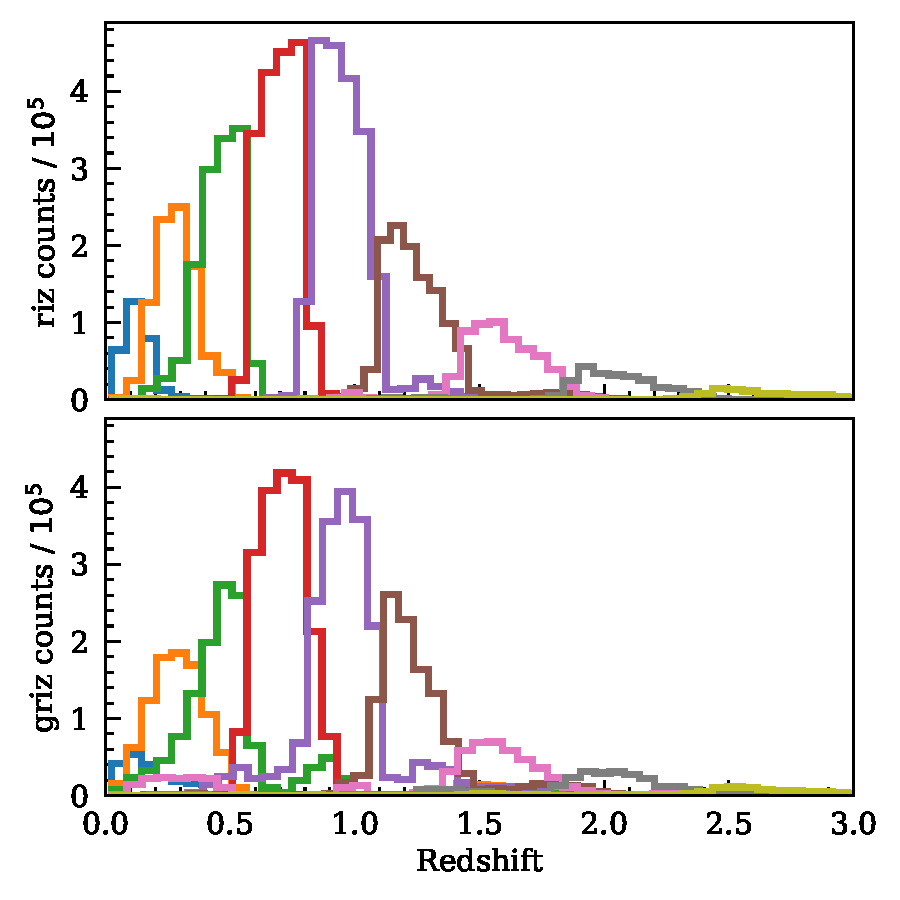
\includegraphics[width=1\linewidth]{results/funbins_nz.pdf}
\caption{$n(z)$ values from funbins}
\label{fig:funbin_nz}
\end{figure}



\subsection{Metric comparisons} \label{sec:metric-results}
Figure \ref{fig:metrics} shows a comparison of some of the different metrics used in the challenge.
We plot, using assignments for methods and for all bin counts, the relationship between our fiducial
metric, the DETF 3x2pt on CosmoDC2, and other metrics we measured.

\begin{enumrate}
\item Generally good relationship, especially at high end
\item Domination of metric by clustering
\item Bimodality in SNR
\end{enumerate}

\begin{figure}[htbp]
% \centering
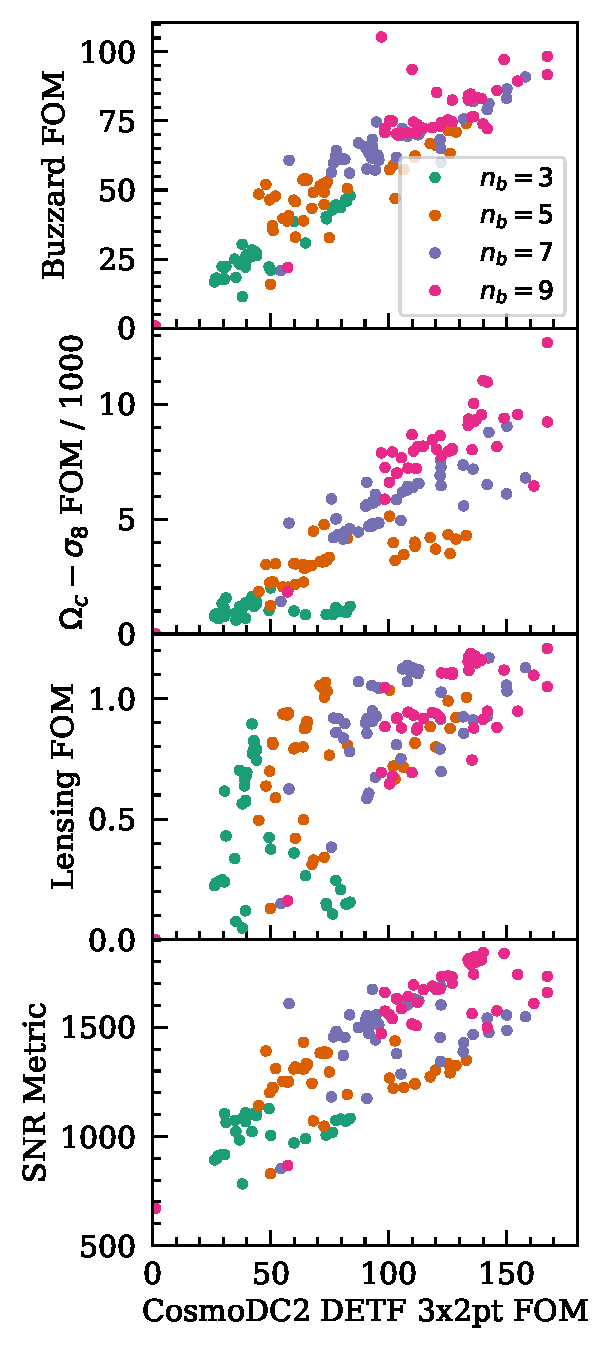
\includegraphics[width=0.9\linewidth]{results/metric_comparisons.pdf}
\caption{A comparison of the metrics used in our challenge. The x-axis is shared, and shows
the 3x2pt $w_0 - w_a$ (DETF) figure of merit on the CosmoDC2 data set for all methods, 
with colours labelling the number
of bins used.  Each of the panels shows a metric which is the same except for a single change, 
which is labelled on its y-axis.  For example, the top panel still shows the 3x2pt $w_0 - w_a$ (DETF) figure of merit,
but for the Buzzard data set.}
\label{fig:metrics}
\end{figure}



\subsection{Impact of losing g-band} \label{sec:gband}
Figure \ref{fig:loss} shows the ratio of the FOM between methods using the griz and the same method
using the riz.  Each point represents one method with a specific number of bins, indicated by colour.
For lower scoring methods and for smaller numbers of bins there is more scatter in the ratio,
but for the highest scoring algorithms and configurations the loss when losing g-band is a little
more stable, at around 10--15\%.

This is true in particular for the highest scoring methods, so we may assume the behaviour to be
generic. The value of the extra FoM that could be gained should be weighed against 
the challenge of high-accuracy
PSF measurement for this band, and the cost in time and effort of determining it, 
but until the end of the survey this is unlikely to be the limiting factor in overall precision.


\begin{figure*}
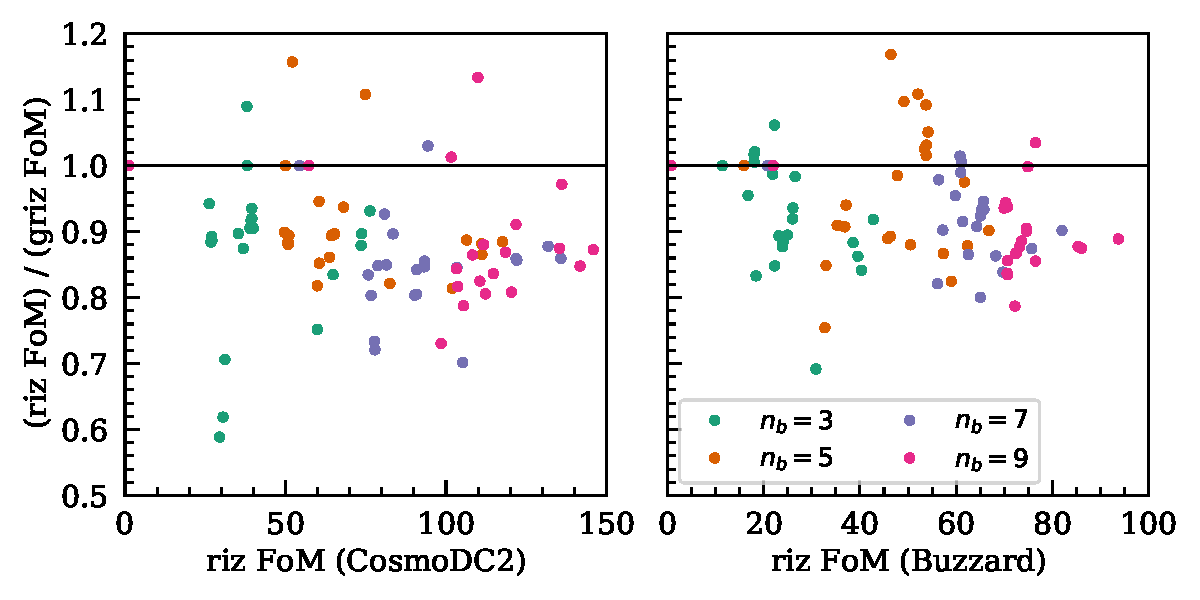
\includegraphics[width=0.9\linewidth]{results/g_band_loss.pdf}
\caption{The degradation in constraining power over all methods
 when comparing them on methods including and excluding
the g-band, in terms of the ratio of the $w_0-w-a$ figure of merit.  The left-hand panel shows
results for the CosmoDC2 scenarios, and the right-hand panel for the Buzzard scenarios.  Colours
indicate the number of bins used in the analysis.}
\label{fig:loss}
\end{figure*}

\subsection{Trained edges vs fixed edges}

Some of the methods in the challenge accepted target bin edges as an input to their algorithms,
and then used classifiers to assign objects to those bins.  Other methods optimized the values
of bin edges themselves, by optimizing the metric.  For the runs shown here, these methods all
targeted one of the 3x2pt metrics. \textbf{Check this is correct}.

A comparison of trained-edge and fixed-edge methods on the CosmoDC2 griz scenarios
is shown in Figure \ref{fig:edges}.  One important point to note is that while trained-edge
methods dominate the highest scores for the 3x2pt DETF metric, on which they trained, they
fare much worse on the lensing-only metrics (the methods were not re-trained on the lensing metrics;
we show the metrics for the same assigned bins).  This suggests that the difference between
optimal bins for different science cases is a significant one, and thus that analysis pipelines
should make it straightforward to calibrate multiple configurations and pass them to
subsequent science anlysis.

\begin{figure*}
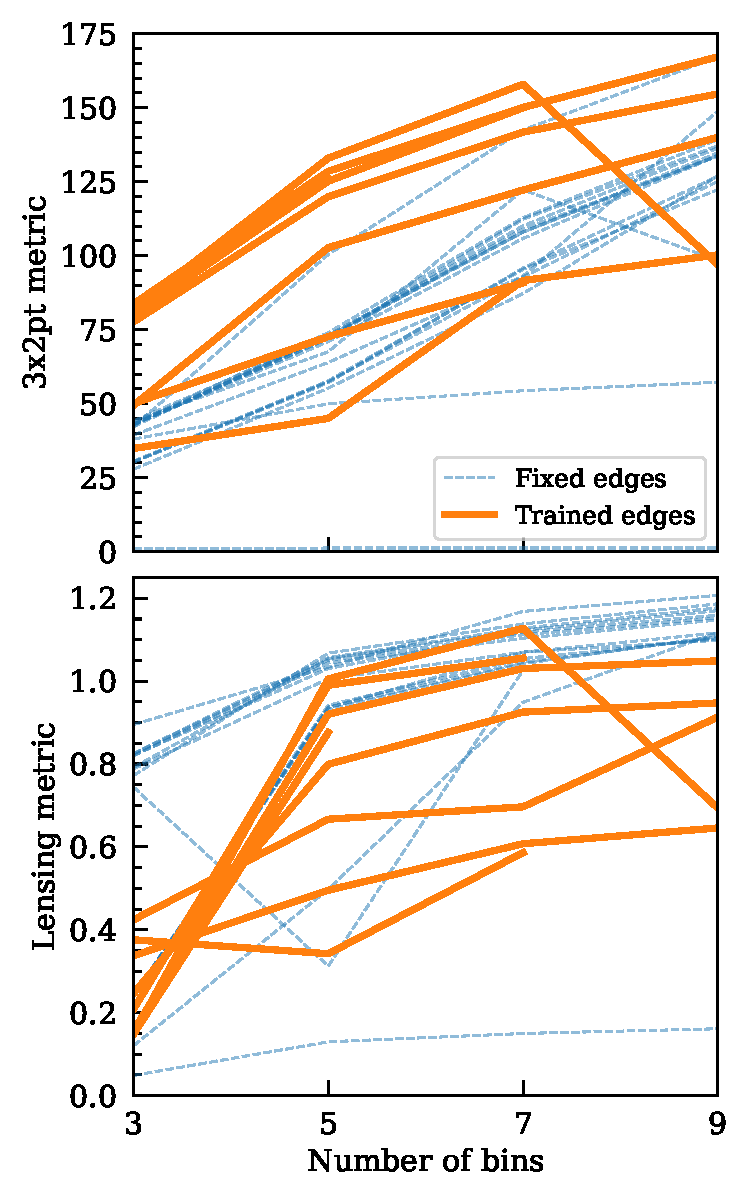
\includegraphics[width=0.9\columnwidth]{results/edge_comparison.pdf}
\caption{A comparison of results from methods which used fixed target edges (dashed blue)
with those which optimized target bins (solid orange).  Methods were trained on the 3x2pt metric
shown in the upper panel; the lower performance for these classifications 
for the lensing-only metric shown in the lower panel illustrates the need for science case-specific
binning choices. In each case, classification is done using griz bands on the CosmoDC2 data set.}
\label{fig:edges}
\end{figure*}

Among methods with fixed bins, those using equal numbers in each tend to plateau at scores of
120-140 in Table \ref{tab:cosmodc2}, suggesting that a range of machine learning models can
effectively classify by bin, at least in this case of representative, extensive training
information.  Notably, this is the case even for the UTOPIA entry, which uses the nearest 
training set neighbour to assign bins and thus was explicitly designed to work only
for this idealised scenario; it should give an upper limit when using the same fixed bins.
That other methods with the same nominal bin choice acheive scores close to it once again
confirms that many entries are close to the best possible score for this approach.


Several of the methods with optimized target bin edges break this
barrier and acheive very high scores.  This included ZotNet, JaxResNet, and JaxCNN.  The
Stacked Generalization method similarly included manually tuned bin edges to maximize
score for this scenario. The typical 15--20\% improvement in FoM scores when optimizing
nominal bin edges makes clear that this easy win should is compelling.

Notably, though, the method that received the highest overall score in Table \ref{tab:cosmodc2}, 
{\sc funbins} did so with a simpler approach - it used a random forest to assign galaxies to bins,
but chose nominal bin edges using an equal width bins in \emph{comoving distance} $\chi$, converting
this to redshift using a fiducial cosmology. The success of this simple solution suggests this
as an easy heuristic for well-optimized nominal edges.




\subsection{Future directions}

\begin{itemize}
    \item spectroscopic incompleteness / unrepresentativeness
    \item data set volume
    \item comparison of optimal choices in different science cases
\end{itemize}


\section{Acknowledgements}
ESC acknowledges support from the FAPESP (\#2019/19687-2) and CNPq  (\#308539/2018-4).

\bibliography{paper}


\appendix

\section{Theory}\label{app:theory}

In our metrics, the power spectrum between two tomographic bins $i$ and $j$ is
computed using either the Core Cosmology Library \citep{ccl} or the JAX
Cosmology Library \citep{jax-cosmo} as:

\begin{equation}
    C^{ij}_\ell = \int_0^{\infty} \frac{q_i(\chi) q_j(\chi)}{\chi^2} P\left(\frac{\ell +\frac{1}{2}}{\chi}, \chi \right) \mathrm{d}\chi
\end{equation}
where $\chi = \chi(z)$ is the comoving distance and $P$ the non-linear matter power spectrum at
a fiducial cosmology.  The kernel functions $q_i(\chi)$ are different for the lensing and clustering samples:
\begin{align}
    q^{\mathrm{cluster}}_i(\chi) &= n_i(\chi)\\
    q^{\mathrm{lensing}}_i(\chi) &= \frac{3}{2}\Omega_m \left(\frac{\mathrm{H}_0}{c}\right)^2 \frac{\chi}{a(\chi)} \int_\chi^{\infty} \frac{\chi' - \chi}{\chi'} n_i(\chi')\,\,\mathrm{d}\chi'
\end{align}
where $n_i(\chi) = n_i(z) \frac{\mathrm{d}z}{\mathrm{d}\chi}$.

We evaluate these at 100 $\ell$ values from $\ell_\mathrm{min}=100$ to $\ell_\mathrm{max}=2000$.

We use a Gaussian estimate for the covariance \citep{takada_jain}; this also incorporates the number of galaxies in the
sample:
\begin{equation}
    \mathrm{Cov}(C^{ij}_\ell, C^{mn}_\ell) = \frac{1}{(2 \ell + 1)\Delta\ell f_\mathrm{sky}}(D^{im}_\ell + D^{jn}_\ell)(D^{in}_\ell + D^{jm}_\ell)
\end{equation}
where $D^{ij}_\ell = C^{ij}_\ell + N^{ij}_\ell$ and we assume an $f_\mathrm{sky}=0.25$.  The noise spectra are:
\begin{align}
N^{\mathrm{cluster},ij}_\ell = \delta_{ij} / n_i \\
N^{\mathrm{lensing},ij}_\ell = \delta_{ij} \sigma_e^2 / n_i
\end{align}
where $n_i$ is the number density of galaxies in bin $i$ (we asssume equally weighted galaxies, and a 
total number density over all bins of 20 galaxies per square arcminute) and $\sigma_e=0.26$.

\section{Complete results}
\label{sec:complete}

\begin{table*}[]
\begin{tabular}{|l|llll|llll|}
                & \multicolumn{4}{c|}{\textbf{riz}}      & \multicolumn{4}{c|}{\textbf{griz}}                                \\ \hline
\textbf{Method} & \textbf{3-bin} & \textbf{5-bin} & \textbf{7-bin} & \textbf{9-bin} & \textbf{3-bin} & \textbf{5-bin} & \textbf{7-bin} & \textbf{9-bin} \\ \hline
{\sc Autokeras\_LSTM } & 22.3 & 32.7    & 61.8    & --    & 26.3             & 43.4             & --             & 72.2\\
{\sc CNN } & 18.0 & 36.9    & 59.8    & 70.3    & 17.7             & 40.7             & 62.6             & 74.5\\
{\sc ComplexSOM } & 30.4 & 47.8    & 57.2    & 74.9    & 25.0             & 48.5             & 63.4             & 75.0\\
{\sc ENSEMBLE1 } & 53.8 & 53.8    & 74.6    & 74.6    & 52.2             & 52.2             & 82.9             & 82.9\\
{\sc funbins } & 23.2 & 50.5    & 65.0    & 72.2    & 26.0             & 57.4             & 81.3             & 91.7\\
{\sc GPzBinning } & 16.8 & 46.4    & 61.4    & 70.7    & 17.6             & 39.7             & 67.0             & 82.5\\
{\sc IBandOnly } & 11.4 & 15.9    & 20.8    & 22.0    & 11.4             & 15.9             & 20.8             & 22.0\\
{\sc JaxCNN } & 38.6 & 59.0    & 69.7    & --    & 43.7             & 71.5             & 83.1             & 95.4\\
{\sc JaxResNet } & 39.6 & 61.7    & --    & --    & 45.9             & 63.3             & --             & --\\
{\sc LGBM } & 18.2 & 37.1    & 60.9    & 70.7    & 17.8             & 39.5             & 61.6             & 75.4\\
{\sc LSTM } & 18.0 & 35.3    & 61.1    & 69.9    & 17.9             & 38.8             & 60.9             & 74.7\\
{\sc mlpqna } & 24.1 & 54.2    & 65.7    & 73.2    & 27.2             & 51.5             & 70.4             & 83.4\\
{\sc myCombinedClassifiers } & 18.4 & 33.0    & 56.1    & 85.3    & 22.1             & 38.8             & 68.3             & 97.2\\
{\sc NeuralNetwork1 } & 42.8 & 66.8    & 82.0    & 93.7    & 46.6             & 74.1             & 90.9             & 105.4\\
{\sc NeuralNetwork2 } & 21.9 & 52.1    & 60.8    & 76.5    & 22.2             & 47.0             & 59.9             & 73.9\\
{\sc PCACluster } & 22.3 & 49.2    & 56.4    & --    & 21.0             & 44.8             & 57.6             & --\\
{\sc Random } & 0.8 & 0.8    & 0.8    & 0.8    & 0.8             & 0.8             & 0.8             & 0.8\\
{\sc RandomForest } & 23.9 & 53.4    & 65.0    & 72.5    & 27.3             & 52.1             & 70.4             & 83.5\\
{\sc SimpleSOM } & 26.1 & 46.3    & 64.3    & 70.7    & 28.3             & 51.9             & 70.8             & 84.7\\
{\sc TensorFlow\_FFNN } & -- & --    & --    & --    & --             & --             & --             & --\\
{\sc TCN } & 26.6 & 53.7    & 65.7    & 74.6    & 27.0             & 49.2             & 69.4             & 82.4\\
{\sc UTOPIA } & 24.9 & 53.8    & 65.3    & 73.6    & 27.9             & 52.9             & 70.1             & 83.1\\
{\sc ZotBin } & 30.8 & 57.4    & 68.2    & 76.5    & 44.6             & 66.2             & --             & 89.4\\
{\sc ZotNet } & 40.3 & 62.4    & 75.7    & 86.0    & 48.0             & 71.0             & 86.6             & 98.4\\
\end{tabular}
\caption{INCOMPLETE, AND AUTO-GENERATED SO NO POINT EDITING! Values of the 3x2pt DETF figure-of-merit achieved by entrant methods on the 
Buzzard part of the challenge.}
\label{tab:buzzard_3x2}
\end{table*}

\begin{table*}[]
\begin{tabular}{|l|llll|llll|}
                & \multicolumn{4}{c|}{\textbf{riz}}      & \multicolumn{4}{c|}{\textbf{griz}}                                \\ \hline
\textbf{Method} & \textbf{3-bin} & \textbf{5-bin} & \textbf{7-bin} & \textbf{9-bin} & \textbf{3-bin} & \textbf{5-bin} & \textbf{7-bin} & \textbf{9-bin} \\ \hline
{\sc Autokeras\_LSTM } & 13.8 & 30.2    & 31.1    & --    & 26.4             & 7.7             & 43.0             & 44.6\\
{\sc CNN } & 7.0 & 29.8    & 37.5    & 38.1    & 6.2             & 35.8             & 45.0             & 48.7\\
{\sc ComplexSOM } & 17.3 & 19.7    & 25.0    & 25.4    & 6.5             & 12.2             & 19.3             & 21.5\\
{\sc ENSEMBLE1 } & 36.0 & 36.0    & 38.6    & *    & *             & *             & *             & *\\
{\sc funbins } & 23.3 & 31.6    & 36.5    & 39.8    & 31.2             & 43.0             & 50.4             & 54.0\\
{\sc GPzBinning } & 6.9 & 23.9    & 33.1    & 35.1    & 6.5             & 36.0             & 46.0             & 47.8\\
{\sc IBandOnly } & 0.8 & 2.6    & 3.2    & 3.6    & 0.8             & 2.6             & 3.2             & 3.6\\
{\sc JaxCNN } & 9.3 & 27.9    & 29.0    & --    & 3.3             & 38.0             & 42.7             & --\\
{\sc JaxResNet } & 2.1 & 30.8    & 37.9    & --    & 2.2             & 31.1             & --             & 44.7\\
{\sc LGBM } & 7.0 & 30.1    & 37.5    & 39.6    & 6.3             & 36.3             & 45.4             & 48.6\\
{\sc LSTM } & 6.9 & 29.3    & 36.8    & 38.2    & 6.4             & 35.5             & 44.6             & 48.9\\
{\sc mlpqna } & 23.1 & 35.0    & 37.3    & 38.0    & 30.0             & 43.9             & 48.9             & 51.4\\
{\sc myCombinedClassifiers } & 1.2 & 8.4    & 28.8    & 39.1    & 1.7             & 10.9             & 37.2             & 49.3\\
{\sc NeuralNetwork1 } & 1.6 & 34.0    & 36.7    & 25.0    & 2.1             & 37.7             & 46.3             & 25.0\\
{\sc NeuralNetwork2 } & 19.2 & 21.8    & 22.4    & 35.8    & 8.5             & 18.6             & 22.5             & 36.7\\
{\sc PCACluster } & 7.8 & 11.3    & 14.2    & *    & 12.6             & 12.0             & 21.6             & *\\
{\sc PQNLD } & 20.2 & 30.9    & 35.0    & 36.4    & 27.6             & 44.4             & 49.9             & 52.9\\
{\sc Random } & 0.0 & 0.0    & 0.0    & 0.0    & 0.0             & 0.0             & 0.0             & 0.0\\
{\sc RandomForest } & 23.5 & 34.9    & 38.4    & 39.6    & 30.0             & 44.5             & 50.1             & 53.2\\
{\sc SimpleSOM } & 20.5 & 30.7    & 35.1    & 36.7    & 28.8             & 45.4             & 50.7             & 53.8\\
{\sc TensorFlow\_FFNN } & 22.6 & 34.4    & 36.7    & 37.7    & 29.7             & 43.4             & 48.3             & 50.9\\
{\sc TCN } & 23.6 & 36.0    & 38.0    & 38.7    & 27.6             & 41.2             & 46.3             & 49.4\\
{\sc UTOPIA } & 22.0 & 31.1    & 35.1    & 36.3    & 29.8             & 43.2             & 49.6             & 52.3\\
{\sc ZotBin } & 4.8 & 24.8    & 30.9    & 29.1    & 4.0             & 27.3             & 35.9             & 38.1\\
{\sc ZotNet } & 2.2 & 29.9    & 33.1    & 34.6    & 2.3             & 33.2             & 42.3             & 43.0\\

\end{tabular}
\caption{INCOMPLETE, AND AUTO-GENERATED SO NO POINT EDITING! Values of the weak lensing $\Omega_c - \sigma_8$
figure-of-merit achieved by entrant methods on the CosmoDC2 part of the challenge.}
\label{tab:dc2_wl}
\end{table*}

\begin{table*}[]
\begin{tabular}{|l|llll|llll|}
                & \multicolumn{4}{c|}{\textbf{riz}}      & \multicolumn{4}{c|}{\textbf{griz}}                                \\ \hline
\textbf{Method} & \textbf{3-bin} & \textbf{5-bin} & \textbf{7-bin} & \textbf{9-bin} & \textbf{3-bin} & \textbf{5-bin} & \textbf{7-bin} & \textbf{9-bin} \\ \hline
{\sc Autokeras\_LSTM } & 2.9 & 10.5    & 8.2    & --    & 5.7             & 5.0             & --             & 11.5\\
{\sc CNN } & 1.8 & 9.5    & 12.3    & 13.2    & 1.8             & 9.4             & 14.7             & 16.2\\
{\sc ComplexSOM } & 1.9 & 6.2    & 7.5    & 8.4    & 1.0             & 7.9             & 13.2             & 15.9\\
{\sc ENSEMBLE1 } & 11.4 & 11.4    & 13.7    & 13.7    & 13.9             & 13.9             & 17.9             & 17.9\\
{\sc funbins } & 4.4 & 8.8    & 10.8    & 11.8    & 7.2             & 13.1             & 16.3             & 17.4\\
{\sc GPzBinning } & 1.7 & 9.3    & 11.3    & 12.5    & 2.1             & 10.6             & 15.0             & 16.7\\
{\sc IBandOnly } & 0.2 & 0.3    & 0.4    & 0.4    & 0.2             & 0.3             & 0.4             & 0.4\\
{\sc JaxCNN } & 4.0 & 10.0    & 11.6    & --    & 4.4             & 13.1             & 14.9             & 15.5\\
{\sc JaxResNet } & 4.2 & 10.2    & --    & --    & 4.8             & 11.3             & --             & --\\
{\sc LGBM } & 1.8 & 9.5    & 12.5    & 13.4    & 1.8             & 9.6             & 14.5             & 16.5\\
{\sc LSTM } & 1.8 & 9.6    & 12.6    & 13.3    & 1.9             & 9.6             & 14.5             & 16.5\\
{\sc mlpqna } & 4.8 & 11.2    & 13.0    & 13.7    & 6.9             & 13.8             & 17.3             & 18.3\\
{\sc Stacked Generalization } & 1.5 & 6.6    & 11.0    & 13.1    & 2.3             & 9.5             & 14.9             & 17.6\\
{\sc NeuralNetwork1 } & 3.9 & 10.2    & 12.0    & 13.3    & 5.0             & 14.5             & 16.4             & 17.9\\
{\sc NeuralNetwork2 } & 2.3 & 9.8    & 11.1    & 12.6    & 2.8             & 7.0             & 9.8             & 14.1\\
{\sc PCACluster } & 3.8 & 6.0    & 4.2    & *    & 1.2             & 2.5             & 5.0             & *\\
{\sc PQNLD } & 4.6 & 10.4    & 11.9    & 12.7    & 6.9             & 14.2             & 17.3             & 18.3\\
{\sc Random } & 0.0 & 0.0    & 0.0    & 0.0    & 0.0             & 0.0             & 0.0             & 0.0\\
{\sc RandomForest } & 4.6 & 10.8    & 12.6    & 13.1    & 6.8             & 13.8             & 17.2             & 18.2\\
{\sc SimpleSOM } & 4.7 & 10.4    & 12.0    & 12.7    & 7.3             & 15.0             & 17.6             & 18.5\\
{\sc FFNN } & 4.7 & 11.0    & 12.8    & 13.5    & 6.8             & 13.7             & 16.8             & 17.7\\
{\sc TCN } & 5.0 & 10.9    & 12.9    & 13.4    & 6.2             & 12.2             & 15.8             & 16.4\\
{\sc UTOPIA } & 4.2 & 9.9    & 11.6    & 12.1    & 6.6             & 13.0             & 16.2             & 17.2\\
{\sc ZotBin } & 5.7 & 8.8    & 10.8    & 10.5    & 3.6             & 10.0             & 11.3             & 12.4\\
{\sc ZotNet } & 3.8 & 10.1    & 11.5    & 11.7    & 4.3             & 11.3             & 13.1             & 13.4\\


\end{tabular}
\caption{INCOMPLETE, AND AUTO-GENERATED SO NO POINT EDITING! Values of the weak lensing $\Omega_c - \sigma_8$
figure-of-merit achieved by entrant methods on the Buzzard part of the challenge.}
\label{tab:buzzard_wl}
\end{table*}

\section{Mistakes}
The challenge organizers made a number of mistakes when building and running the challenge.
These do not invalidate our process or results, but we describe some of them here in the hope of
being useful for future challenge designers.

\subsection{Splitting nominal bin choice from assignment}
There were two ways to obtain good scores in the challenge: either one could choose the best
nominal bin edges, or find the best method to put galaxies into those bins once they are chosen.
These two are not completely disconnected: some theoretically powerful choices of nominal edges
could prove impossible to assign in practice.  But it would still have been useful to separate
the challenge into two separate parts, fixing the edges while optimizing classifiers, and vice
versa.   We can retrospectively determine this since we understand the classifiers, but the picture
would have been clearer doing so in advance.

\subsection{Infrastructure}
Since submissions could use a wide variety of libraries and dependencies, it was extremely
difficult after the challenge was complete to build appropriate environments for all the challenges
in order to run the methods on additional data sets. In retrospect, a robust and careful
continuous integration tool with a mechanism for entrants to specify an environment (for example, a 
container or a {\sc conda} requirements file) could have been used to simplify this and ensure
all methods could be easily run by the organizers.

Once additional issue, though, was that many methods required GPUs to train in a reasonable time,
and specifying an environment on these systems can be more complicated.

\subsection{Guidance on caching \& batch processing}
Since the training process for the challenge could be slow for some algorithms, many entries
(very reasonably) cached trained models or other values for later use.  In some cases these
cached values were then incorrectly picked up by subsequent runs on new data sets, leading
to (at best) crashes and at worst silently poor scores.  We should have provided an explicit
caching mechanism for entrants to avoid such issues.

Additionally, the challenge supplied the data described in Section \ref{sec:data} to entrants,
and some assumed that it was safe to hard-code specific paths to them or
otherwise assume fixed data inputs.  This led to problems when switching to new test data sets. 
Again, a requirement enforced by continuous integration could have checked this.

%=====================
% END OF THE MAIN TEXT
%=====================

\end{document}
